%!TEX root = report.tex

\subsection{Intrinsic Calibration}
\label{sec:intrinsic}

Every camera is characterised by what is called its \textit{intrinsic parameters}. They consist of the focal width and height, $f_x$ and $f_y$, and the principal point $\begin{bmatrix} c_x &  c_y\end{bmatrix}$ which is usually at the image center. These parameters are grouped in the camera matrix $C$ as

\begin{align}
    C &= \begin{bmatrix}
        f_x & 0 & c_x \\
        0 & f_y & c_y \\
        0 & 0 & 1 \\
    \end{bmatrix}.
\end{align}

Furthermore, every camera creates some radial and tangential distortion in the images which needs to be taken into account. 
If $x'$ and $y'$ are the coordinates of the undistorted image points normalized with $z$ such that $z'=1$ and centered around the principal point $c_x$ and $c_y$, then the distorted points $x''$ and $y''$ can be modelled using Brown-Conrady's decentering distortion model \cite{Brown1966}, \cite{Conrady1919}
\begin{align}
    x'' &= x' k(r) + (2p_1 x' y' + p_2(r^2 + 2x'^2))(1+p_3r^2+p_4r^4 + \cdots) \\
    y'' &= y' k(r) + (p_1(r^2+2y'^2) + 2p_2x'y')(1+p_3r^2+p_4r^4 + \cdots) \\
    \text{with} \quad k(r) &= 1+k_1r^2+k_2r^4 + \cdots \text{  and } r^2=x'^2+y'^2.
\end{align}

The distortion coefficients are indifferent to the camera resolution \cite{calib3d}, only the focal width and height and the principal point have to be scaled appropriately. To reduce imprecisions due to scaling, a recalibration was done every time the camera resolution was changed.

An algorithm for finding the intrinsic parameters including the radial distortion coefficients was suggested by Zhang \cite{Zhang2000}. 
Its implementation in the \texttt{Matlab Camera Calbiration Toolbox} added an estimation algorithm for two tangential distortion coefficients. \cite{MTB}
The \texttt{OpenCV} implementation used in this project is based on the \texttt{Matlab} Toolbox. 
It is implemented for the first six radial distortion coefficients $r_i$ and the first two tangential distortion coefficients $p_i$ \cite{calib3d}.

The principle of the algorithm is to find the position of chessboard corners in an image and to match them to their object coordinates. For good functioning, this needs to be repeated for various postions of the checkerboard, as shown in Figures \ref{fig:checkerboard}

\begin{figure}[H]
    \centering
    \begin{subfigure}{0.2\linewidth}
        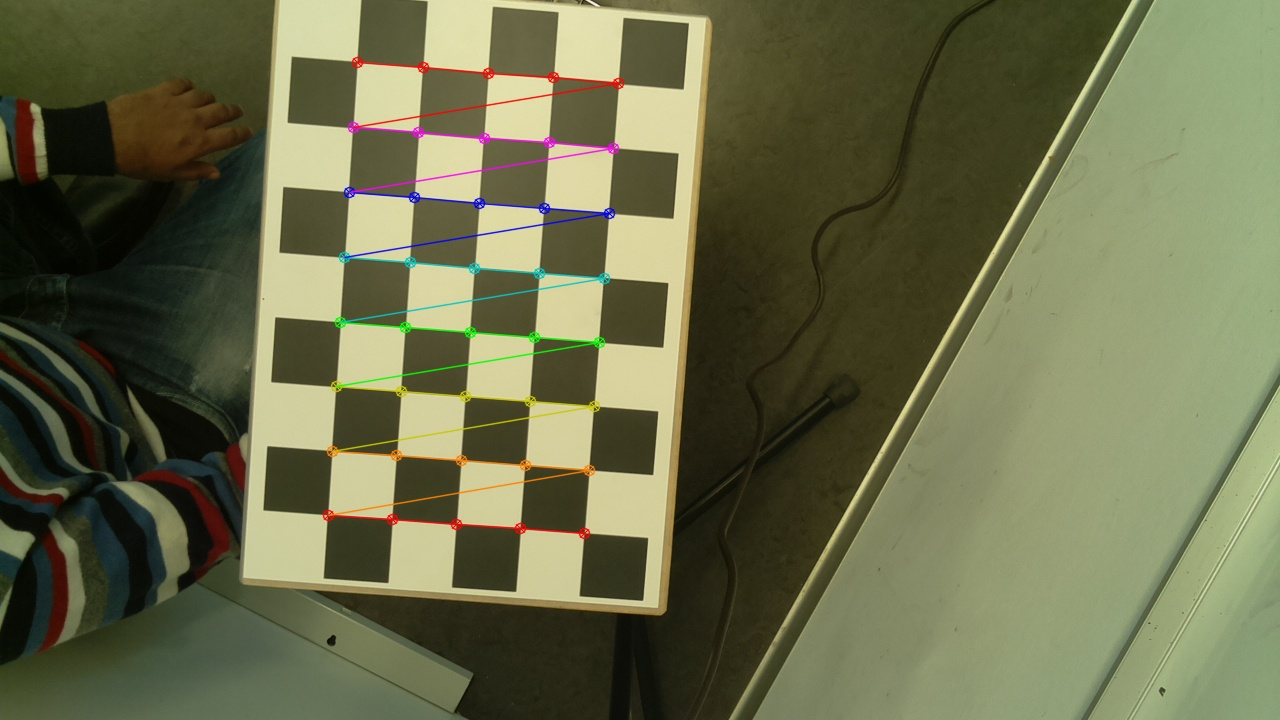
\includegraphics[width=\linewidth]{files/output145_1.jpg}
    \end{subfigure} 
    \begin{subfigure}{0.2\linewidth}
        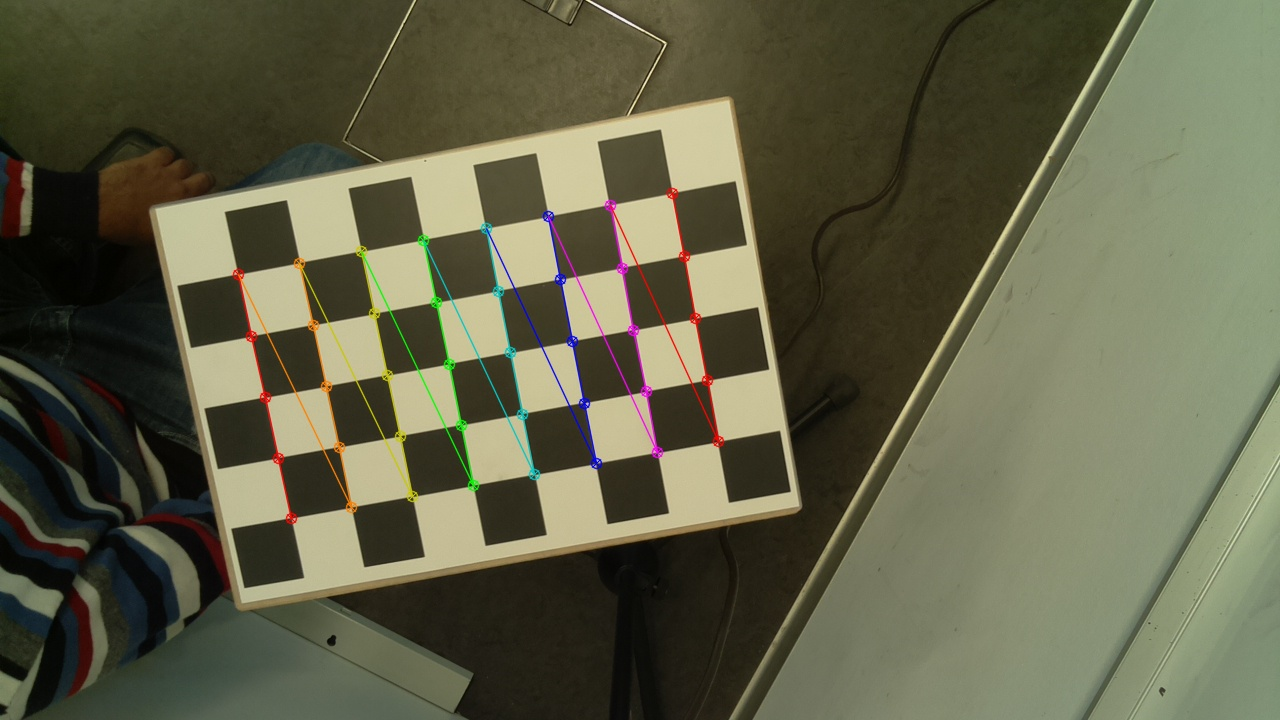
\includegraphics[width=\linewidth]{files/output145_2.jpg}
    \end{subfigure}
    \begin{subfigure}{0.2\linewidth}
        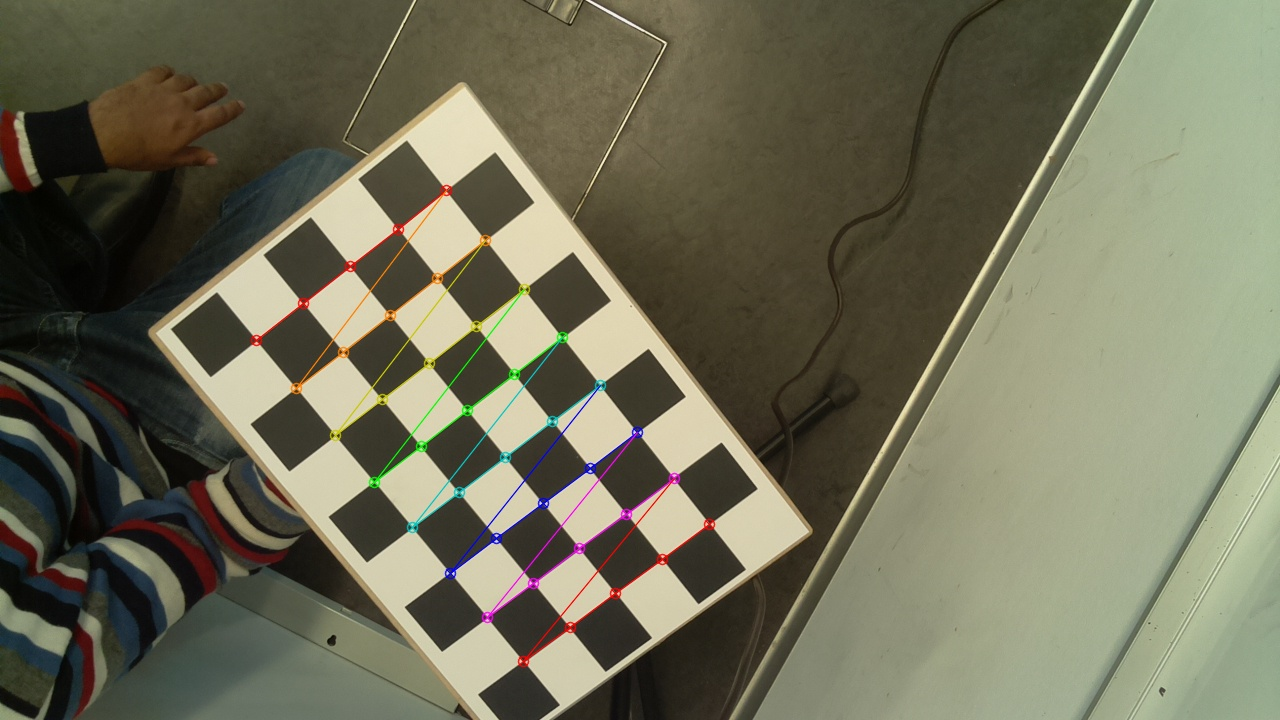
\includegraphics[width=\linewidth]{files/output145_3.jpg}
    \end{subfigure}
    \begin{subfigure}{0.2\linewidth}
        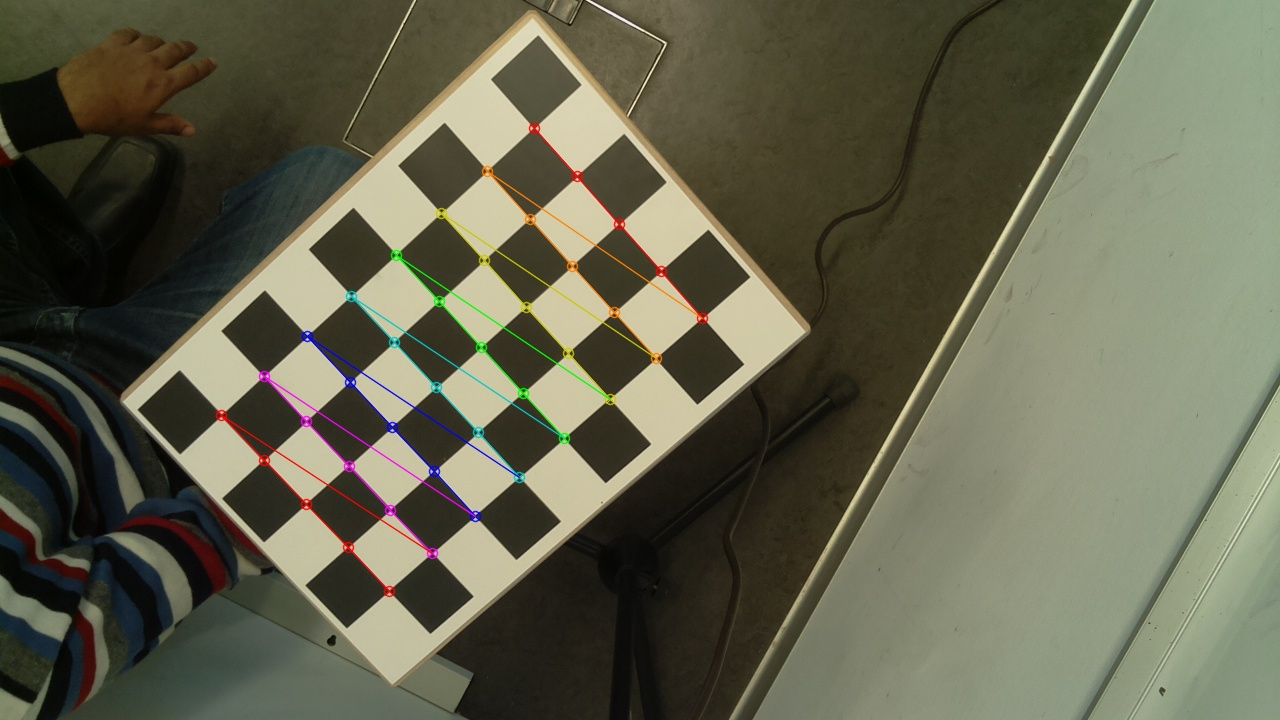
\includegraphics[width=\linewidth]{files/output145_4.jpg}
    \end{subfigure} \\
    \begin{subfigure}{0.2\linewidth}
        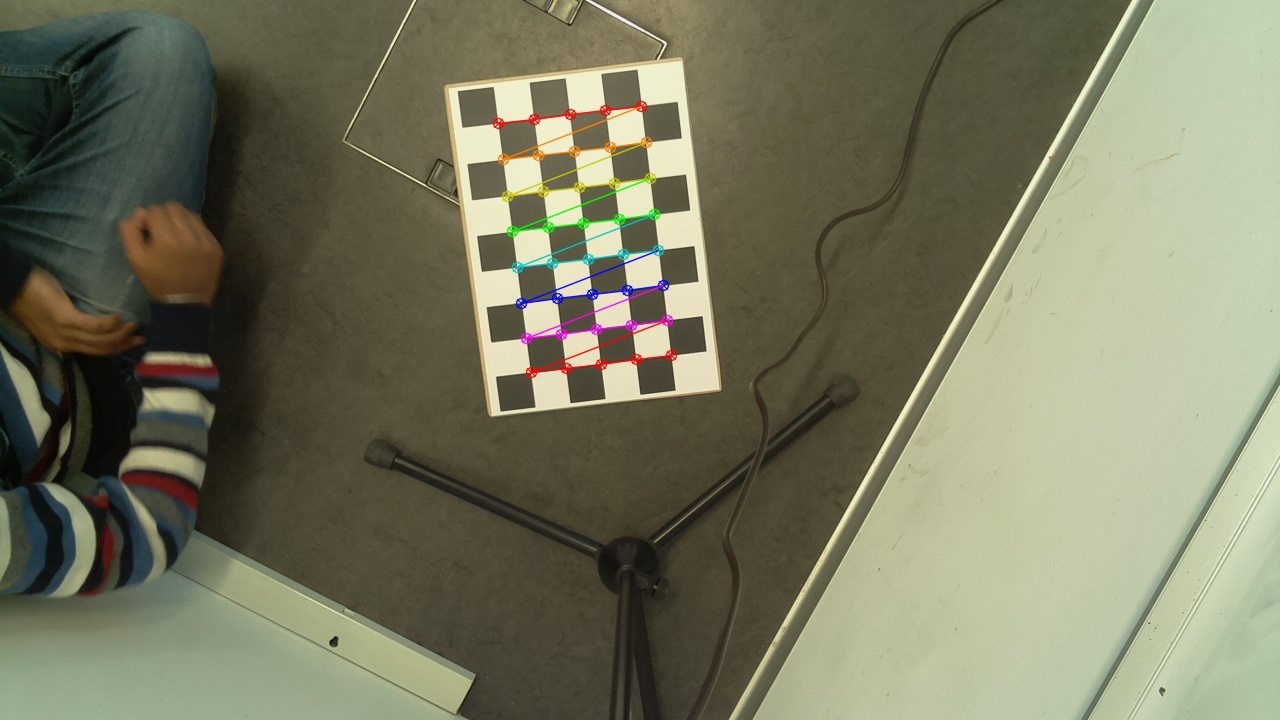
\includegraphics[width=\linewidth]{files/output145_5.jpg}
    \end{subfigure}
    \begin{subfigure}{0.2\linewidth}
        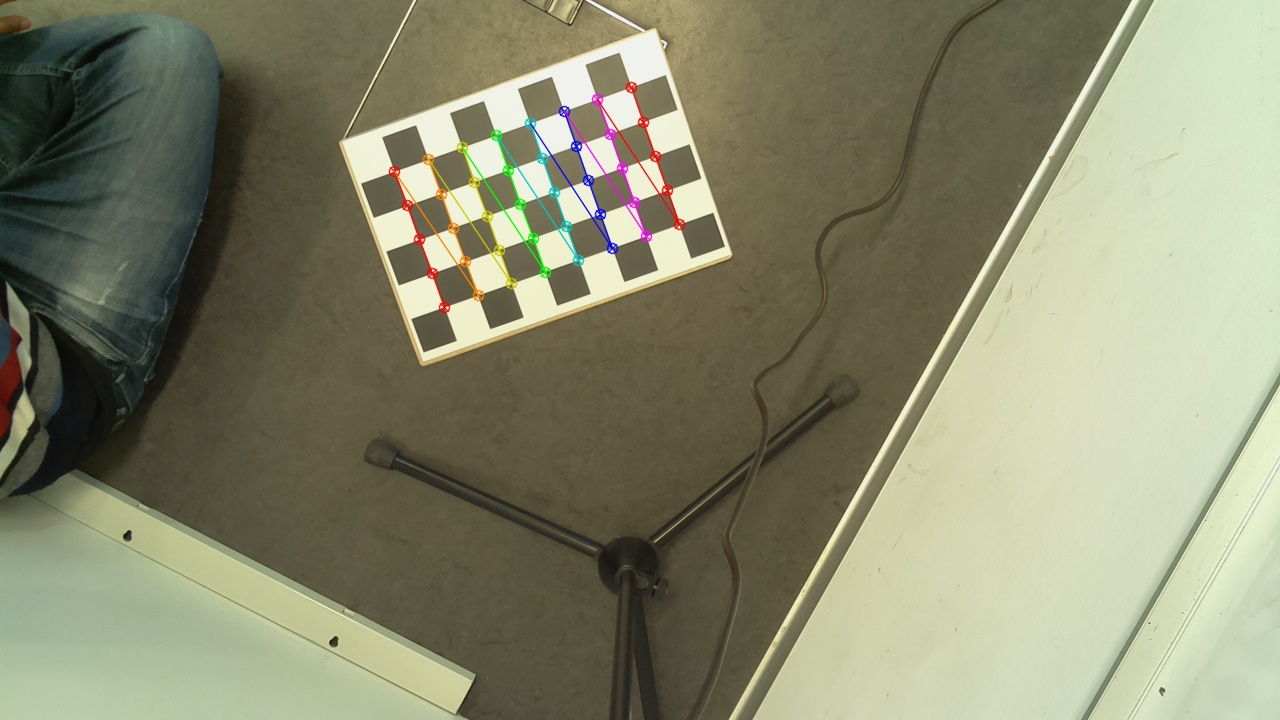
\includegraphics[width=\linewidth]{files/output145_6.jpg}
    \end{subfigure}
    \begin{subfigure}{0.2\linewidth}
        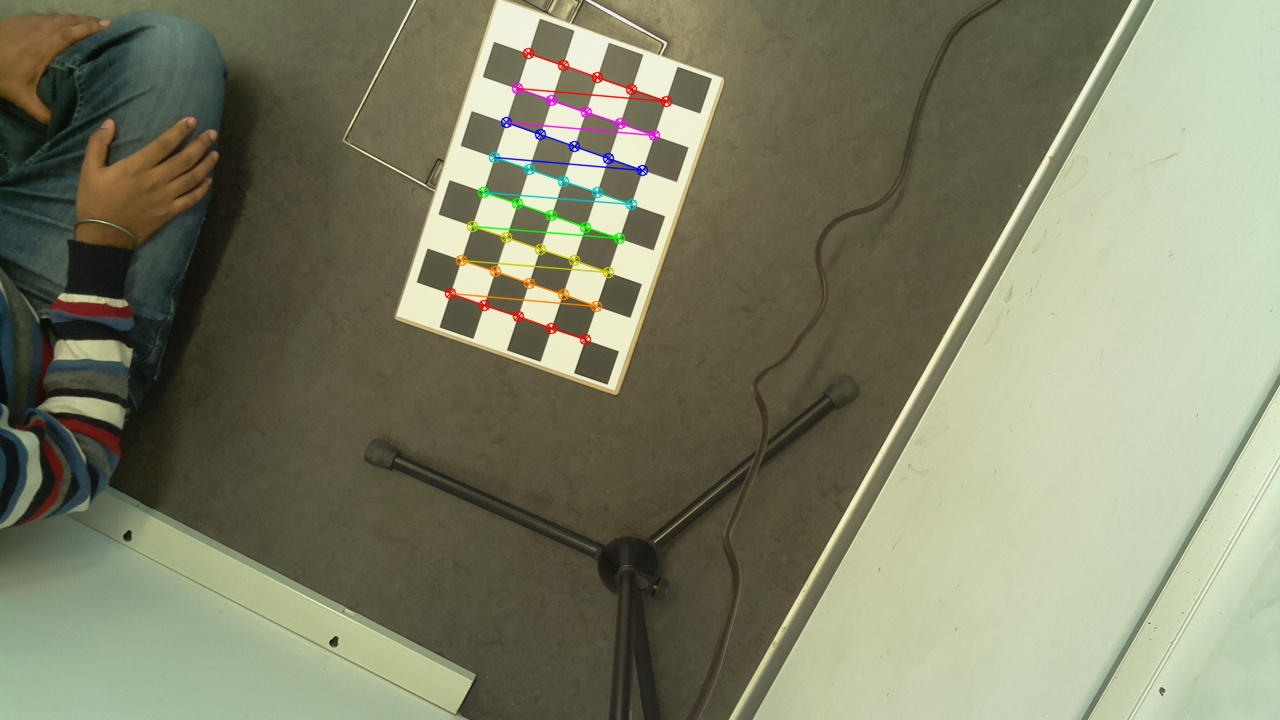
\includegraphics[width=\linewidth]{files/output145_7.jpg}
    \end{subfigure}
    \begin{subfigure}{0.2\linewidth}
        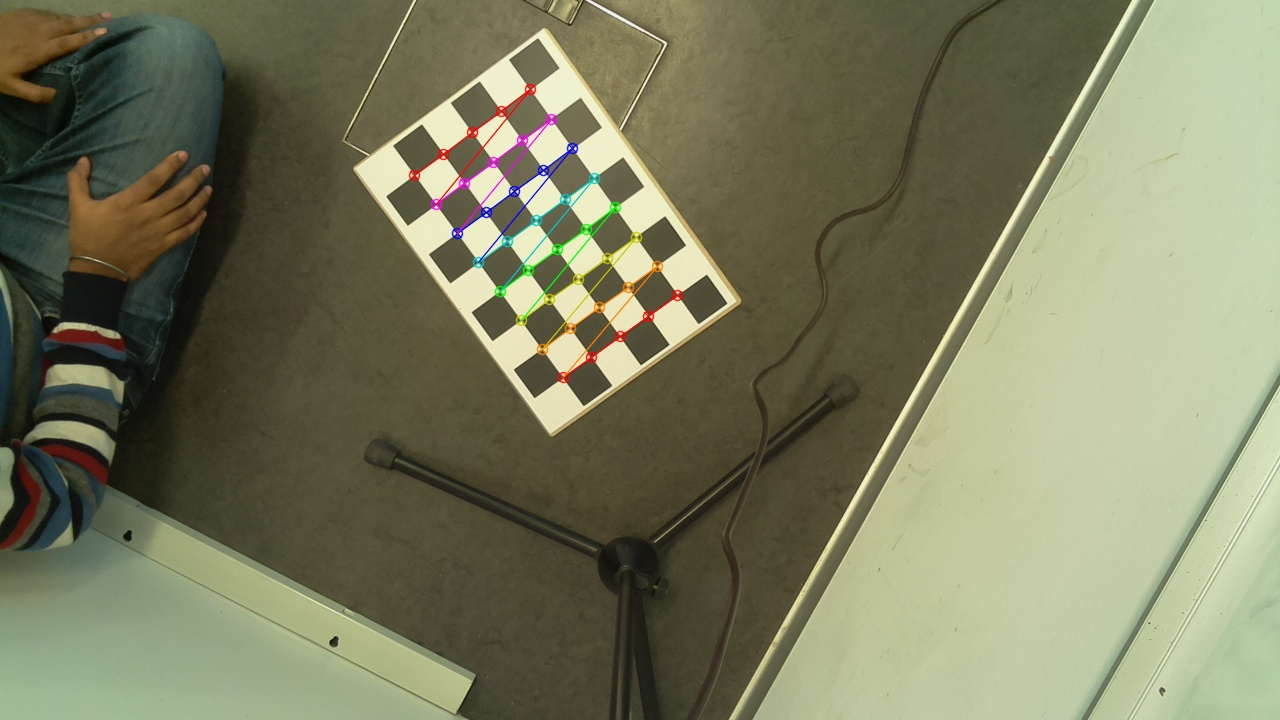
\includegraphics[width=\linewidth]{files/output145_8.jpg}
    \end{subfigure}
    \caption{Checkerboard images used for intrinsic calibration. }
    \label{fig:checkerboard}
\end{figure}

To ensure correct results, it is tested whether the obtained coefficients are close enough to what is given by the manufacturer. 
We have the following relation between the focal length, the image resolution and the sensor size

\begin{equation}
    f_x = \frac{w \times f_{x,mm}}{w_{CCD}} = \frac{1280\text{ px} \times 3.6\text{ mm}}{3.67\text{ mm}} = 1255 \text{ px},
\end{equation}

where $f_{x,mm}$ is the focal width in mm and $w_{CCD}$ is the width of hte CCD sensor, given by the manufacturer.
The obtained pixel value is allowed to be 100 px off this reference value.
% QUESTION: where does the opencv implementation come from??
%$\quad k(r) &=\frac{1+k_1r^2+k_2r^4+k_3r^6}{1+k_4r^2+k_5r^4+k_6r^6} $
